\documentclass{article}

%% Page Margins %%
\usepackage{geometry}
\geometry{
    top = 0.75in,
    bottom = 0.75in,
    right = 0.75in,
    left = 0.75in,
}

\usepackage{amsmath}
\usepackage{graphicx}
\usepackage{parskip}

\title{Assembly Project: Dr Mario}

\author{Aakaash Rohra}

\begin{document}
\maketitle

\section{Introduction}
The project was recreating the NES game Dr. Mario in MIPS Assembly. I implemented the core mechanics (milestones 1-3) as well as 8 additional features (milestones 4/5) that I will go through in this report.
\begin{enumerate}
    \item Which milestones were implemented? \\
    Milestone 1: Drawing the scene \\ Milestone 2: Movement and other controls \\ Milestone 3: Collision detection + falling logic \\ Milestone 4/5: Game features
    \item How to view the game:
    \begin{enumerate}
    \item 1x1 unit width/height (pixels)
    \item 32x32 display width/height (pixels)
    \item Base Address for Display: 0x10008000 (\$gp)
    \end{enumerate}
\end{enumerate}

\section{Milestones and Features}
\begin{figure}[ht!]
    \centering
    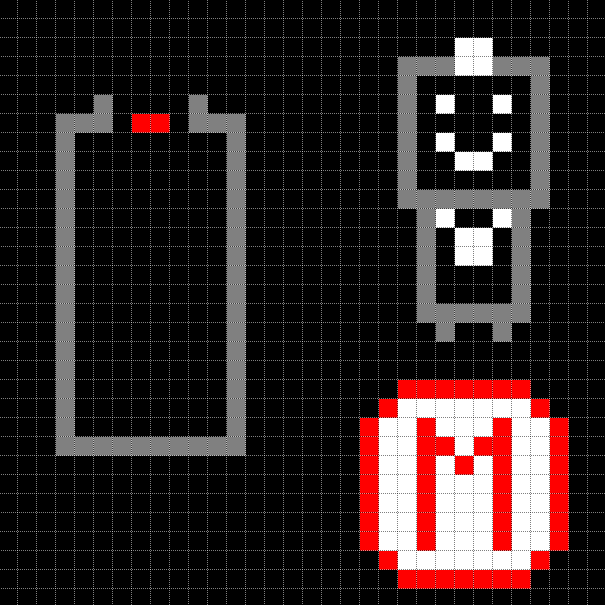
\includegraphics[width=0.2\textwidth]{plan.png}
    \caption{Original Plan for Bitmap Display}
    \label{Instructions}
\end{figure}

\begin{enumerate}
\item Milestone 1: I handled drawing the map by storing into .data the objects to be drawn. Each object consisted of the following in order: 4 bytes for the width, 4 bytes for the height, 4 bytes for the starting position on the bitmap display (in pixels), and then the rest of the object was an array in order of colours that make up the image -- left to right, top to bottom. That way, the same function to draw an image onto the bitmap display could be reused for different images.
\item Milestone 2: Movement from keyboard input was handled similarly to the example given to us. Before rotating the capsule upon pressing 'w', and before shifting the capsule left or right, I made sure that the capsule could be moved without hitting a wall. If it couldn't, nothing happened - return to game loop. To make the capsule move, it was erased (replaced with black) from the bitmap display and the two pixels below the capsule were replaced with the capsule colours instead.
\item Milestone 3: When the player presses 's' to move the capsule down, if it cannot move down, a collision occurs. The capsule colours are stored into the array for play area data, and the addresses for each half of the capsule in the PLAY AREA DATA array is stored into the CAPSULES array so that it can be known which blocks belong to the same capsule (each group of 8 bytes/two blocks in the CAPSULES arrray is one capsule). Storing this information is important for implementing falling logic. When any collision occurs, horizontal and vertical line checks of 4 or more begin. If they exist, they are deleted (replaced with black), and the corresponding addresses in the CAPSULES array replaced with 0. Now, capsules above the blocks that are gone that are entirely unsupported must fall, and any capsules missing one half (so only one half remaining) have that half drop as well. The first 4 spots (16 bytes) in the CAPSULES array are reserved for the viruses, as those are single blocks, yet must not fall even with empty space below them.
\item Milestones 4/5: Below are the features I implemented.
\end{enumerate}

(1) Implement gravity, so that each second that passes will automatically move the capsule down one row.\\
(2) Have the speed of gravity increase gradually over time.\\\\
On each sleep call, a counter increments by that many milliseconds (16 ms in my case). When this counter exceeds the set limit, the current capsule falls by one pixel, and the set limit decreases slightly (so it is reached slightly faster next time).\\\\
(4) When the player has reached the ”game over” condition, display a Game Over screen in pixels on the screen. Restart the game if a “retry” option is chosen by the player.\\\\
The game over screen loops until either 'y' is pressed to play again, or 'q' to quit the game. If the player presses 'y', a loop starts to replace the entire inside of the glass bottle with black again (effectively resetting the game). The CAPSULES array is not reset as the entire game restarts, and values are overwritten from the start of the array. Any leftover values are effectively garbage and it does not matter if they continue to technically exist within the array, as they would not cause any issues if they do happen to be detected at some point.\\\\
(5) Add sound effects for different conditions (rotating, moving, placing, completing 4+, blocked action, game over, and new game).\\\\
Sound effects were implemented with the syscall 31, and some short durations and notes in the .data section for each different sound.\\\\
(6) If the player presses the keyboard key p, display a ”Paused” message on screen until they press p a second time, at which point the original game will resume.\\\\
Upon pressing 'p', a pause loop begins that only breaks upon pressing 'p' again to unpause. A pause symbol is drawn in the lower left corner of the bitmap display.\\\\
(7) Add levels to the game that trigger after the player eliminates all of the viruses in the current level. The next level should be more difficult than the previous one.\\\\
I opted to increase the speed between levels as a means of making the new level more difficult. When it is detected that all 4 viruses are set to 0/black in internal data, the glass bottle is reset to black and the set limit for the millisecond counter to reach before dropping the capsule by 1 pixel is reduced dramatically.\\\\
(13) Draw Dr. Mario and the viruses on the side panels.\\
(14) Have each virus image disappear as the viruses of that colour are eliminated from the playing field.\\\\
The virus colours are stored into a VIRUS DATA array at the same time that they are generated and stored into the first 16 bytes of the CAPSULES array. As they are stored in the same order, when it is found that the capsules array has a virus at a certain location set to 0/black, the same index (basically) can be set to black in the VIRUS DATA array. The VIRUS DATA array is formatted as an array that can be drawn using the draw function, and is placed to the right of the play area.\\\\
\begin{figure}[ht!]
    \centering
    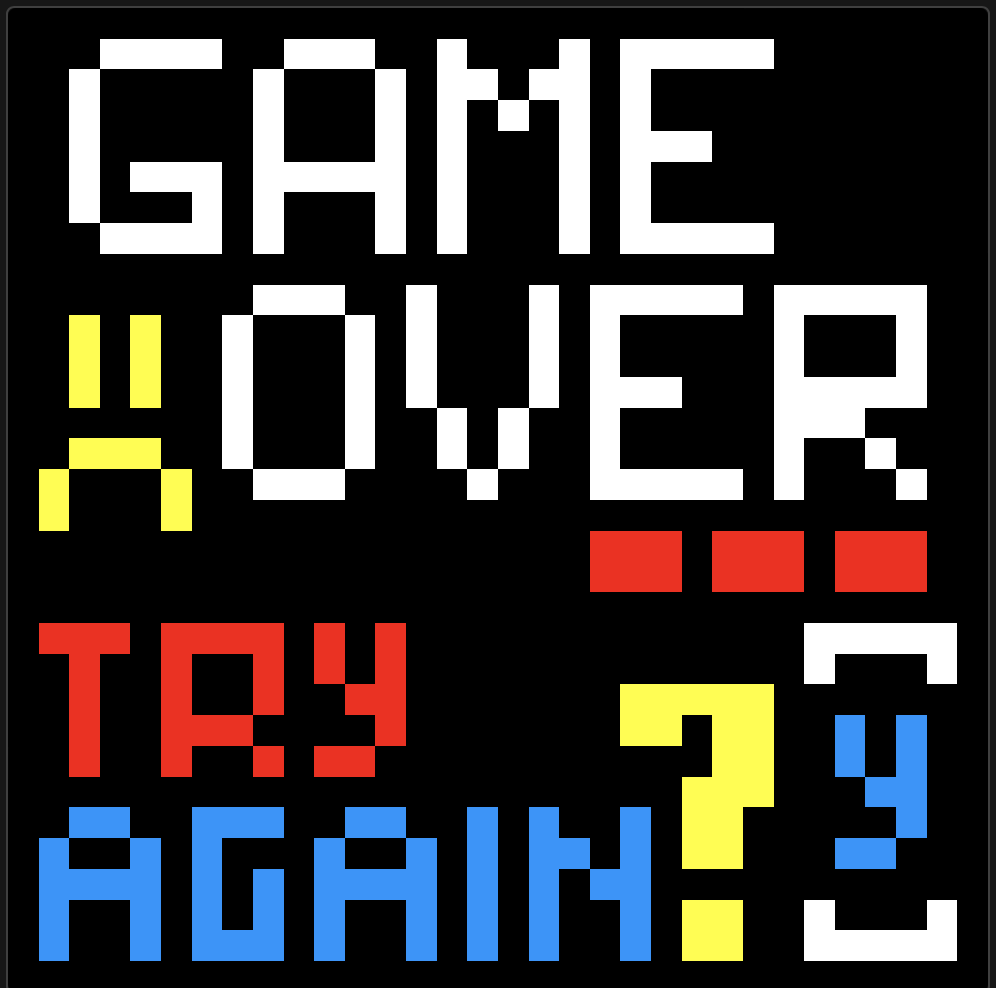
\includegraphics[width=0.2\textwidth]{game_over_screen.png}
    \caption{Feature 4 Game Over Screen}
    \label{Instructions}
\end{figure}
\begin{figure}[ht!]
    \centering
    
\includegraphics[width=0.2\textwidth]{pause.png}
    \caption{Feature 6 Paused}
    \label{Instructions}
\end{figure}
\begin{figure}[ht!]
    \centering
    
\includegraphics[width=0.2\textwidth]{drmario_and_viruses.png}
    \caption{Feature 13 Draw Dr. Mario and the Viruses}
    \label{Instructions}
\end{figure}
\begin{figure}[ht!]
    \centering
    
\includegraphics[width=0.2\textwidth]{viruses_gone.png}
    \caption{Feature 14 Virus Images Disappear}
    \label{Instructions}
\end{figure}

\section{How to Play}
w: Rotate capsule 90 degrees counter-clockwise.\\
a: Move capsule left.\\
s: Move capsule down.\\
d: Move capsule right.\\
p: Pause and unpause the game.\\
y: start a new game from the game over screen.\\
q: quit the game.\\

\section{Conclusions/Discussions}
The largest issue I ran into while coding the game in Assembly was register management - I was not always clean and well organized with my registers, which meant I often found myself running out of them (largely due to the number of global values to keep track of). Planning everything out before even beginning to code would have helped prevent this. Overall though, I am happy with how my implementation of the game turned out - it works as it should, with a fair number and variety of features, and I was able to work my way through tricky issues with handling memory and keeping track of the right addresses (and thus, information) throughout the various states of the game.

\end{document}